\subsection{Fluxions Identification} \label{chapter5:flx:compiler}

The source language for this transformation is of higher-order to allow the modularity required for productivity. 
Moreover, it is implemented as an event-loop to impose the developer to define the causality between asynchronous operations.
% Javascript is such a language and is often implemented on top of an event-loop, like in \textit{Node.js}.
The compiler transforms a \textit{Node.js} application into a fluxional application compliant with the execution model described in section \ref{chapter4:flx-model}.
The chain of compilation is described in figure \ref{fig:compilation}.

\begin{figure}%
  \bigfig{%
    \centering%
    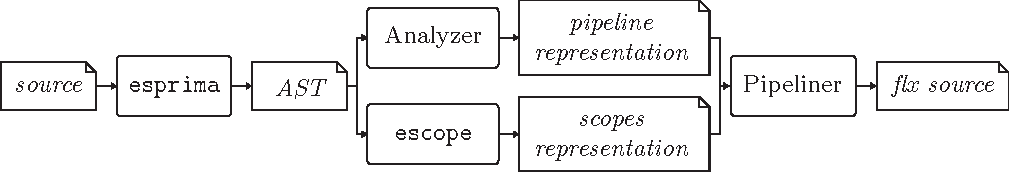
\includegraphics[width=\textwidth]{../resources/compiler-stream.pdf}%
    \caption{Compilation chain}%
    \label{fig:compilation}%
  }%
\end{figure}

The compiler uses the \textit{estools}\ftnt{https://github.com/estools} suite to parse (\texttt{esprima}), analyze (\texttt{escope}), manipulate (\texttt{estraverse} and \texttt{esquery}) and generate (\texttt{escodegen}) source code from an Abstract Syntax Tree (AST).
It is tailored for -- but not limited to -- web applications using \textit{Express}\ftnt{http://expressjs.com/}, the most used \textit{Node.js} web framework.
The compiler extracts an AST from the source with \texttt{esprima}.
From this AST, the \textit{Analyzer} step identifies the rupture points between the different application parts. % and how they relate to form a pipeline.
This first step outputs a pipeline representation of the application.
% Section \ref{chapter5:flx-compiler:analyzer} explains this first compilation step.
In this pipeline representation, the stages are not yet independent and encapsulated into fluxions.
From the AST, \texttt{escope} produces a representation of the memory scopes.
The \textit{Pipeliner} step, explained in section \ref{chapter5:flx:isolation}, analyzes the pipeline representation and the scopes representation to distribute the shared memory into independent groups of fluxions.
% Section \ref{chapter5:flx-compiler:pipeliner} explains this second compilation step.

% \subsubsection{Analyzer step} \label{chapter5:flx-compiler:analyzer}

% The limit between two application parts is defined by a rupture point.
% The analyzer identifies the rupture points, and outputs a representation of the application in a pipeline form.
% Application parts are the stages, and rupture points are the message streams of this pipeline.

\subsubsection{Detection}

In \textit{Node.js}, I/O operations are asynchronous functions and indicate rupture points between two application parts.
Figure \ref{fig:basicrp} shows a code example of a rupture point with the illustration of the execution of the two application parts isolated into fluxions.
The two application parts are the caller of the asynchronous function call on one hand, and the callback provided to the asynchronous function call on the other hand.

\begin{figure}[h!]%
  \bigfig{~}
  \vspace{-2.6\baselineskip}
  \begin{code}
asyncCall(arguments, function callback(result){ //@\circled{2}@ });
// Following statements //@\circled{1}@
  \end{code}%
  \bigfig{%
    \centering
    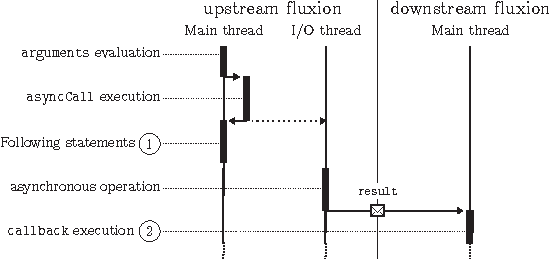
\includegraphics[width=\textwidth]{../resources/basicrp.pdf}%
    \caption{Rupture point interface}%
    \label{fig:basicrp}%
  }%
\end{figure}

Similarly as in the Due compiler, the detection of asynchronous callees is done by the developer. 
It uses a list of common asynchronous callees, like the \texttt{express} and file system methods.
This list can be augmented to match asynchronous callees individually for any application.
To identify the callee, the analyzer walks the AST to find a call expression matching this list.

After the identification of the callee, the callback needs to be identified as well to be encapsulated in the downstream fluxion.
For each asynchronous call detected, the compiler tests if one of the arguments is of type \texttt{function}.
The callback functions declared \textit{in situ} are trivially detected in the AST.
The compiler discard callbacks not declared \textit{in situ}, to avoid altering the semantic by moving or modifying their definitions.
% For variable identifiers, and other expressions, the analyzer tries to detect their type.
% The analyzer walks back the AST to track their assignations and modifications, so as to determine their last value.





% \comment{TODO insert this}
% We developed the compiler core in node.js Javascript.
% There already exist sets of tools for manipulating code in Javascript.
% We used the Esprima suite of tools.